% 名城大学理工学部情報工学科卒業研究発表会
% ・名城大学理工学研究科情報工学専攻公聴会
% アブストラクトサンプル
% Last Update: 2021/11/13

\documentclass[a4paper]{jarticle}
\usepackage{ieabst}
\usepackage{newenum}
\usepackage[dvipdfmx]{graphicx}

%タイトルが長い場合は,勝手に改行されます.
%% 「\\」の挿入で任意の位置に改行を入れられます.
\題目{アブストラクト作成の手引き}
\学籍番号{2XX4XXXXX}
\氏名{名城 太郎}
\研究室{**}
% 旭研究室 宇佐見研究室 亀谷研究室 川澄研究室 小中研究室
% 佐川研究室 鈴木研究室 高比良研究室 田中研究室 寺本研究室
% 中野研究室 野崎研究室 坂野研究室 水沼研究室 向井研究室
% 柳田研究室 山田(啓)研究室 山田(宗)研究室 山本研究室
% 吉川研究室 米澤研究室


%1ページに入りきらない場合は,下の数字を少し小さめに変更.
\renewcommand{\baselinestretch}{1}

\begin{document}
\small

\twocolumn[\vspace*{29mm}] %タイトルが2行の場合は29mm→36mmに.
\begin{論文概要}           %この行は消してはいけません

\section{用紙およびページ数}
卒業研究発表会アブストラクト(学部4年生)はA4用紙1ページ,
修士論文公聴会アブストラクト(大学院修士2年生)はA4用紙2ページ
になります.

\section{執筆要領}

\subsection{マージン}
マージンは以下を目安として,設定してください.

\begin{itemize}
\item 上マージン:30mm
\item 下マージン:27mm
\item 左マージン:25mm
\item 右マージン:25mm
\item カラム間マージン:7mm
\end{itemize}

\subsection{タイトル情報}
上部に以下のタイトル情報をページ全体にわたってセンタリングして1段組で記述してください.

\begin{itemize}
\item タイトル
\item 学籍番号と氏名
\item 所属研究室
\end{itemize}

\subsection{本文}
本文は2段組で記述してください.

本文は,必要に応じて節に分けて記述してください.
ただし,2 レベルまでとし,1, 1.1, 1.2, … のようにナンバリングしてください.

\subsection{図表}
図および表には,図1,表1のような通し番号と,名称を記述してください.ただし,図の場合には図の下部に,表の場合は表の上部に記述してください.

\subsection{参考文献}
参考文献は,本文内で\cite{paper1}\cite{paper2}のように引用し,本文に続いて,参照した文献のリストを掲載してください.参考文献は原則として以下のように記してください.

\begin{newenumerate}

\item {\bf 雑誌の場合}

著者: 標題, 雑誌名, 巻, 号, ページ (発行年).

\item {\bf 単行本の場合}

著者: 書名, ページ数, 発行所 (発行年).

\end{newenumerate}

\section{テンプレートおよびスタイルファイル}
Microsoft Word用のテンプレートと,\LaTeX 用のスタイルファイルを用意してあります.
招待を受けたGoogle Classroomからダウンロードして利用してください.

\subsection{Word用テンプレート}
マージンおよび以下のスタイルが登録してありますので,使ってください.
\begin{itemize}
\item アブストラクトタイトル
\item アブストラクト著者
\item アブストラクト所属
\item アブストラクト見出し1(1,2,3,...)
\item アブストラクト見出し2(1.1, 1.2, ...)
\item アブストラクト見出し3 ((1), (2),…)
\item アブストラクト本文
\item アブストラクト箇条書き(これ)
\item アブストラクト文献見出し(「参考文献」)
\item アブストラクト文献
\end{itemize}

\subsection{\LaTeX 用のスタイルファイル}
以下のように指定してください.

\begin{verbatim}
\documentclass[a4paper,9pt]{jarticle}
\usepackage{ieabst}
\usepackage{newenum}
\usepackage[dvipdfmx]{graphicx}
\end{verbatim}

newenum.styは,Wordテンプレートのスタイル「アブストラクト見出し3((1), (2),…)」に相当するものです.enumerate環境と同様に以下のように使用してください.
\begin{verbatim}
\begin{newenumerate}
\item {\bf アブストラクト見出し}
・・・
\end{newenumerate}
\end{verbatim}

その他は通常のコマンドを使って執筆してください.
そのほかの注意事項は,サンプルファイルを参照してください.

また,.latexmk ファイルを同梱したので,latexmk コマンド一発でコンパイルできます.

\section{PDFファイルについて}

Word,\LaTeX とも,PDFファイルを提出してください.
Wordの場合はdocxファイルを,\LaTeX
の場合はコンパイルに必要なソースファイル・図のファイルをまとめて圧縮したZIPファイル(特殊なスタイルファイルを用いた場合はそれも含める)を同時に提出してください.
WordファイルとPDFファイルについては圧縮する必要はありません.
PDFファイルの作成時は,フォントをすべて埋め込んでください.
また,アブストラクトを白黒プリンタで印刷する場合があり,その場合にカラー画像が見にくくなることを覚悟してください.


\section{\LaTeX 用サンプル}

\subsection{数式のサンプル}

数式のサンプルです.下記の式(\ref{eq:sample1})のように入力します.
\begin{equation}
\label{eq:sample1}
\left\{
\begin{array}{lcl}
\dot{\vec{x}}(t)&=&\vec{A}\vec{x}(t)+\vec{B}\vec{u}(t)\\
\vec{y}(t)&=&\vec{C}\vec{x}(t)
\end{array}
\right.
\end{equation}

\subsection{図表のサンプル}
図および表には,図\ref{fig:sample1},表\ref{tbl:sample1}のような通し番号と,名称を記述してください.ただし,図の場合には図の下部に,表の場合は表の上部に記述してください.

\begin{figure}[ht]
\centering
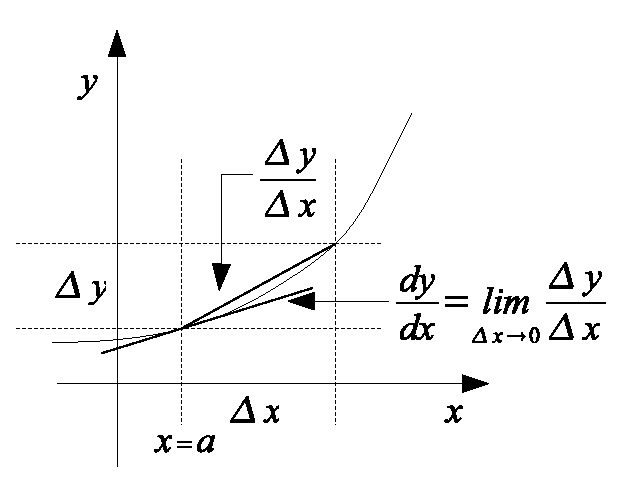
\includegraphics[width=0.9\columnwidth,clip]{2-1.eps}
\caption{EPS図のサンプル}
\label{fig:sample1}
\end{figure}

\begin{figure}[ht]
\centering
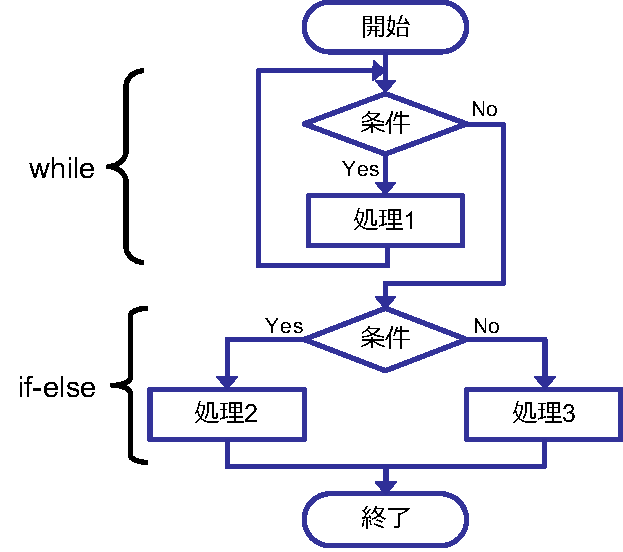
\includegraphics[scale=0.6,clip]{2-2.pdf}
\caption{PDF図のサンプル}
\label{fig:sample2}
\end{figure}

\begin{table}[ht]
\centering
\caption{表のサンプル}
\label{tbl:sample1}
\begin{tabular}{|c|c||c|c|} \hline
$p$ & $q$ & $p\rightarrow q$ & $(p\rightarrow q)\wedge q$ \\ \hline
T & T & T & T \\ \hline
T & F & F & F \\ \hline
F & T & T & T \\ \hline
F & F & T & F \\ \hline
\end{tabular}
\end{table}

\subsection{参考文献のサンプル}
参考文献引用のサンプルです~\cite{paper1}\cite{paper2}.


\begin{thebibliography}{9}
\bibitem{paper1}名城花子, 山田太郎: 卒業論文の書き方に関する検討, 名城情報論文誌,
  Vol.~12, No.~1, pp.~21--28 (2015).
\bibitem{paper2}山本情一, 名城次郎: 卒業研究の進め方の本, p.~301, 名城情報出版 (2009).
\end{thebibliography}

\end{論文概要} %この行は消してはいけません
\end{document}
